\documentclass[12pt]{article}

\usepackage{graphicx}% Include figure files
\usepackage{dcolumn}% Align table columns on decimal point

% Use Arial font %
\usepackage{helvet}
\renewcommand{\familydefault}{\sfdefault} 

% Default margins and paper properties %
\usepackage[a4, portrait, margin=0.6in]{geometry}

\begin{document}
	\title{Hypothesis plots summary} % Force line breaks with \\
	\author{1666957, Gustavo Espinal Lugo}
	\date{\today} % It is always \today, today, %  but any date may be explicitly specified

	\maketitle
	%\tableofcontents
	
	\section*{Plots and corresponding metadata}
	mean expected W mass: 80.379 $[GeV/c^{2}]$,\\
mean hypothesis masses: [78.  78.5 79.  79.5 80.  80.5 81.  81.5 82. ] $[GeV/c^{2}]$,\\
mass width: 2.07 $[GeV/c^{2}]$,\\
chi\_square value of hypothesis fit: 41.682632838592745\\
	Absolute path to figure: /home/physics/phuxdp/Desktop/PX402 Physics Project/WBosonProject/T2W5/plots/muPT\_80.379\_2.07\_between\_78\_and\_82\_summary.png\\
	Next lines are the data of the shown histograms (if needed): \\
	All quantities: 	80.379, [78.  78.5 79.  79.5 80.  80.5 81.  81.5 82. ], 2070, 41.682632838592745\\
	X\_energ\_vls = [0.6, 1.7999999999999998, 3.0, 4.199999999999999, 5.4, 6.6, 7.8, 9.0, 10.2, 11.399999999999999, 12.6, 13.799999999999999, 15.0, 16.2, 17.4, 18.6, 19.799999999999997, 21.0, 22.2, 23.4, 24.6, 25.799999999999997, 27.0, 28.199999999999996, 29.4, 30.6, 31.799999999999997, 33.0, 34.2, 35.4, 36.599999999999994, 37.8, 39.0, 40.2, 41.4, 42.599999999999994, 43.8, 45.0, 46.2, 47.4, 48.599999999999994, 49.8, 51.0, 52.2, 53.4, 54.599999999999994, 55.8, 57.0, 58.199999999999996, 59.4, 60.599999999999994, 61.8, 63.0, 64.19999999999999, 65.4, 66.6, 67.8, 69.0, 70.19999999999999, 71.4, 72.6, 73.8, 75.0, 76.19999999999999, 77.4, 78.6, 79.8, 81.0, 82.19999999999999, 83.4, 84.6, 85.8, 87.0, 88.19999999999999, 89.4, 90.6, 91.8, 93.0, 94.19999999999999, 95.4, 96.6, 97.8, 99.0, 100.19999999999999, 101.4, 102.6, 103.8, 105.0, 106.19999999999999, 107.4, 108.6, 109.8, 111.0, 112.19999999999999, 113.4, 114.6, 115.79999999999998, 117.0, 118.19999999999999, 119.4]\\
	Y\_data\_bin\_cnts = [0.0, 0.0, 0.0, 0.0, 0.0, 0.0, 0.0, 0.0, 0.0, 0.0, 0.0, 0.0, 0.0, 0.0, 0.0, 2.0, 1.0, 22.0, 1489.0, 74358.0, 97268.0, 103398.0, 110581.0, 117586.0, 124146.0, 131104.0, 138550.0, 146457.0, 153167.0, 160283.0, 166239.0, 166552.0, 160112.0, 138916.0, 108363.0, 80056.0, 60365.0, 46302.0, 36320.0, 29356.0, 23917.0, 19684.0, 16134.0, 13535.0, 11629.0, 9812.0, 8341.0, 7057.0, 6261.0, 5391.0, 4703.0, 4022.0, 3551.0, 3209.0, 2798.0, 2519.0, 2255.0, 1986.0, 1795.0, 1653.0, 1479.0, 1359.0, 1181.0, 1055.0, 966.0, 884.0, 775.0, 716.0, 679.0, 629.0, 564.0, 534.0, 440.0, 459.0, 393.0, 399.0, 381.0, 341.0, 309.0, 291.0, 235.0, 242.0, 208.0, 202.0, 184.0, 159.0, 179.0, 166.0, 156.0, 125.0, 120.0, 103.0, 99.0, 98.0, 105.0, 72.0, 83.0, 84.0, 65.0, 69.0]\\
	Y\_model\_bin\_cnts = [0.0, 0.0, 0.0, 0.0, 0.0, 0.0, 0.0, 0.0, 0.0, 0.0, 0.0, 0.0, 0.0, 0.0, 0.9608226418495178, 1.9216463565826416, 3.8432936668395996, 18.255640029907227, 1429.6951904296875, 71774.078125, 92617.7734375, 100092.90625, 106117.984375, 112577.40625, 119587.4453125, 126507.15625, 133990.078125, 140644.796875, 146556.078125, 154044.78125, 158789.4375, 160200.0625, 153735.015625, 133684.125, 103564.7734375, 77319.640625, 57478.203125, 44721.7578125, 35277.66015625, 28096.5703125, 22664.388671875, 18688.986328125, 15737.9443359375, 13054.0478515625, 10866.9541015625, 9428.431640625, 7994.71337890625, 6874.26416015625, 5815.31298828125, 5261.8173828125, 4456.54833984375, 3991.458984375, 3484.08837890625, 3117.972412109375, 2744.17236328125, 2384.784912109375, 2154.162353515625, 1863.0223388671875, 1736.1947021484375, 1559.4046630859375, 1403.752685546875, 1252.9046630859375, 1209.66796875, 1044.4078369140625, 948.3262939453125, 840.7147827148438, 764.810302734375, 716.7696533203125, 634.1396484375, 613.0015258789062, 541.9011840820312, 457.3494567871094, 437.1723937988281, 399.7005310058594, 419.87762451171875, 362.22869873046875, 318.9920959472656, 282.48089599609375, 308.42315673828125, 232.51841735839844, 204.65487670898438, 220.98867797851562, 214.26318359375, 182.55596923828125, 186.39932250976562, 153.73147583007812, 157.57470703125, 153.7314910888672, 126.82865142822266, 121.06363677978516, 116.25952911376953, 110.49457550048828, 86.47396087646484, 115.29866790771484, 84.55236053466797, 86.47403717041016, 86.47406005859375, 75.90495300292969, 67.25758361816406, 51.88441848754883]\\

    Found optimal massses ($\chi^2$ roots): [80.42920702] $[GeV/c^{2}]$
    Uncertainty [GeV/c^2]: 0.05787070778021075

	\begin{figure}[tb]
		\centering
		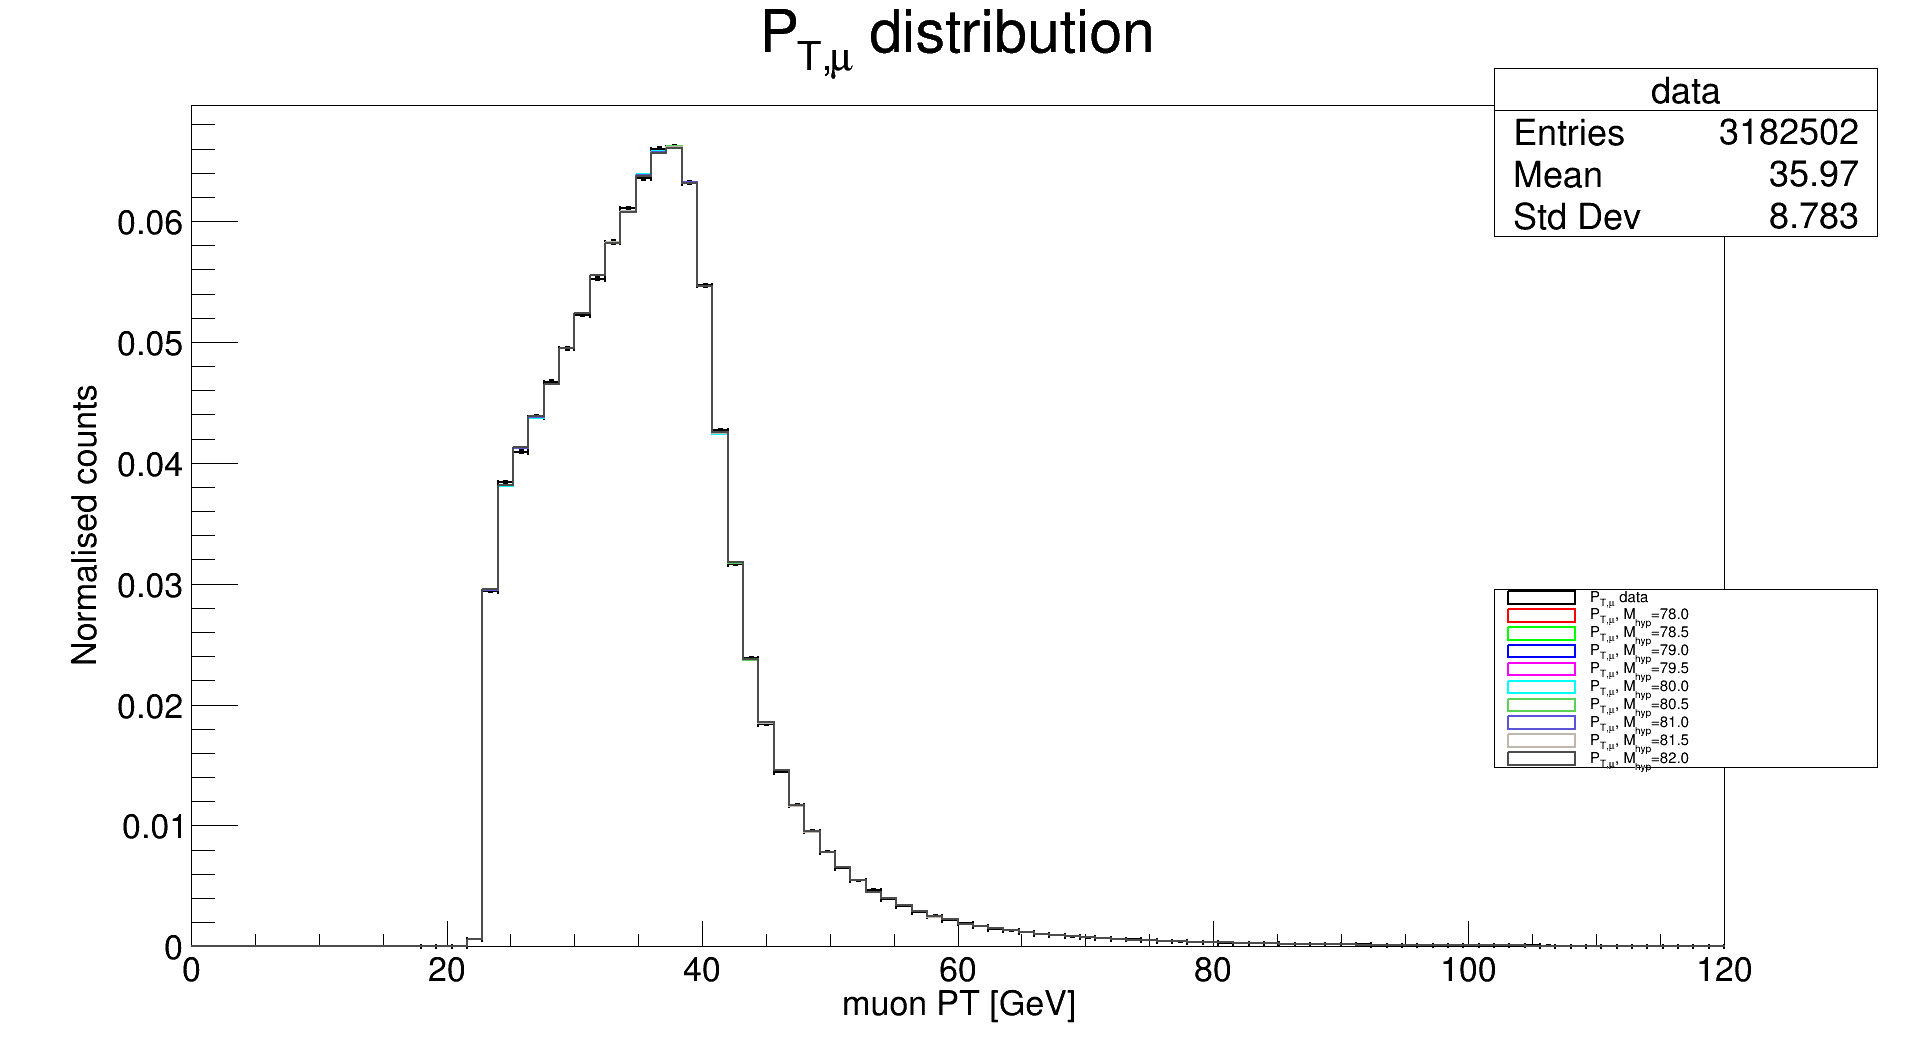
\includegraphics[width=\columnwidth]{/home/physics/phuxdp/Desktop/PX402 Physics Project/WBosonProject/T2W5/plots/muPT_80.379_2.07_between_78_and_82_summary.png}
		\caption{\small Hypothesis masses mean expected W mass: 80.379 $[GeV/c^{2}]$,\\
mean hypothesis masses: [78.  78.5 79.  79.5 80.  80.5 81.  81.5 82. ] $[GeV/c^{2}]$,\\
mass width: 2.07 $[GeV/c^{2}]$,\\
chi_square value of hypothesis fit: 41.682632838592745. }
		\label{fig: fig_0}
	\end{figure}

       \begin{figure}[tb]
		\centering
		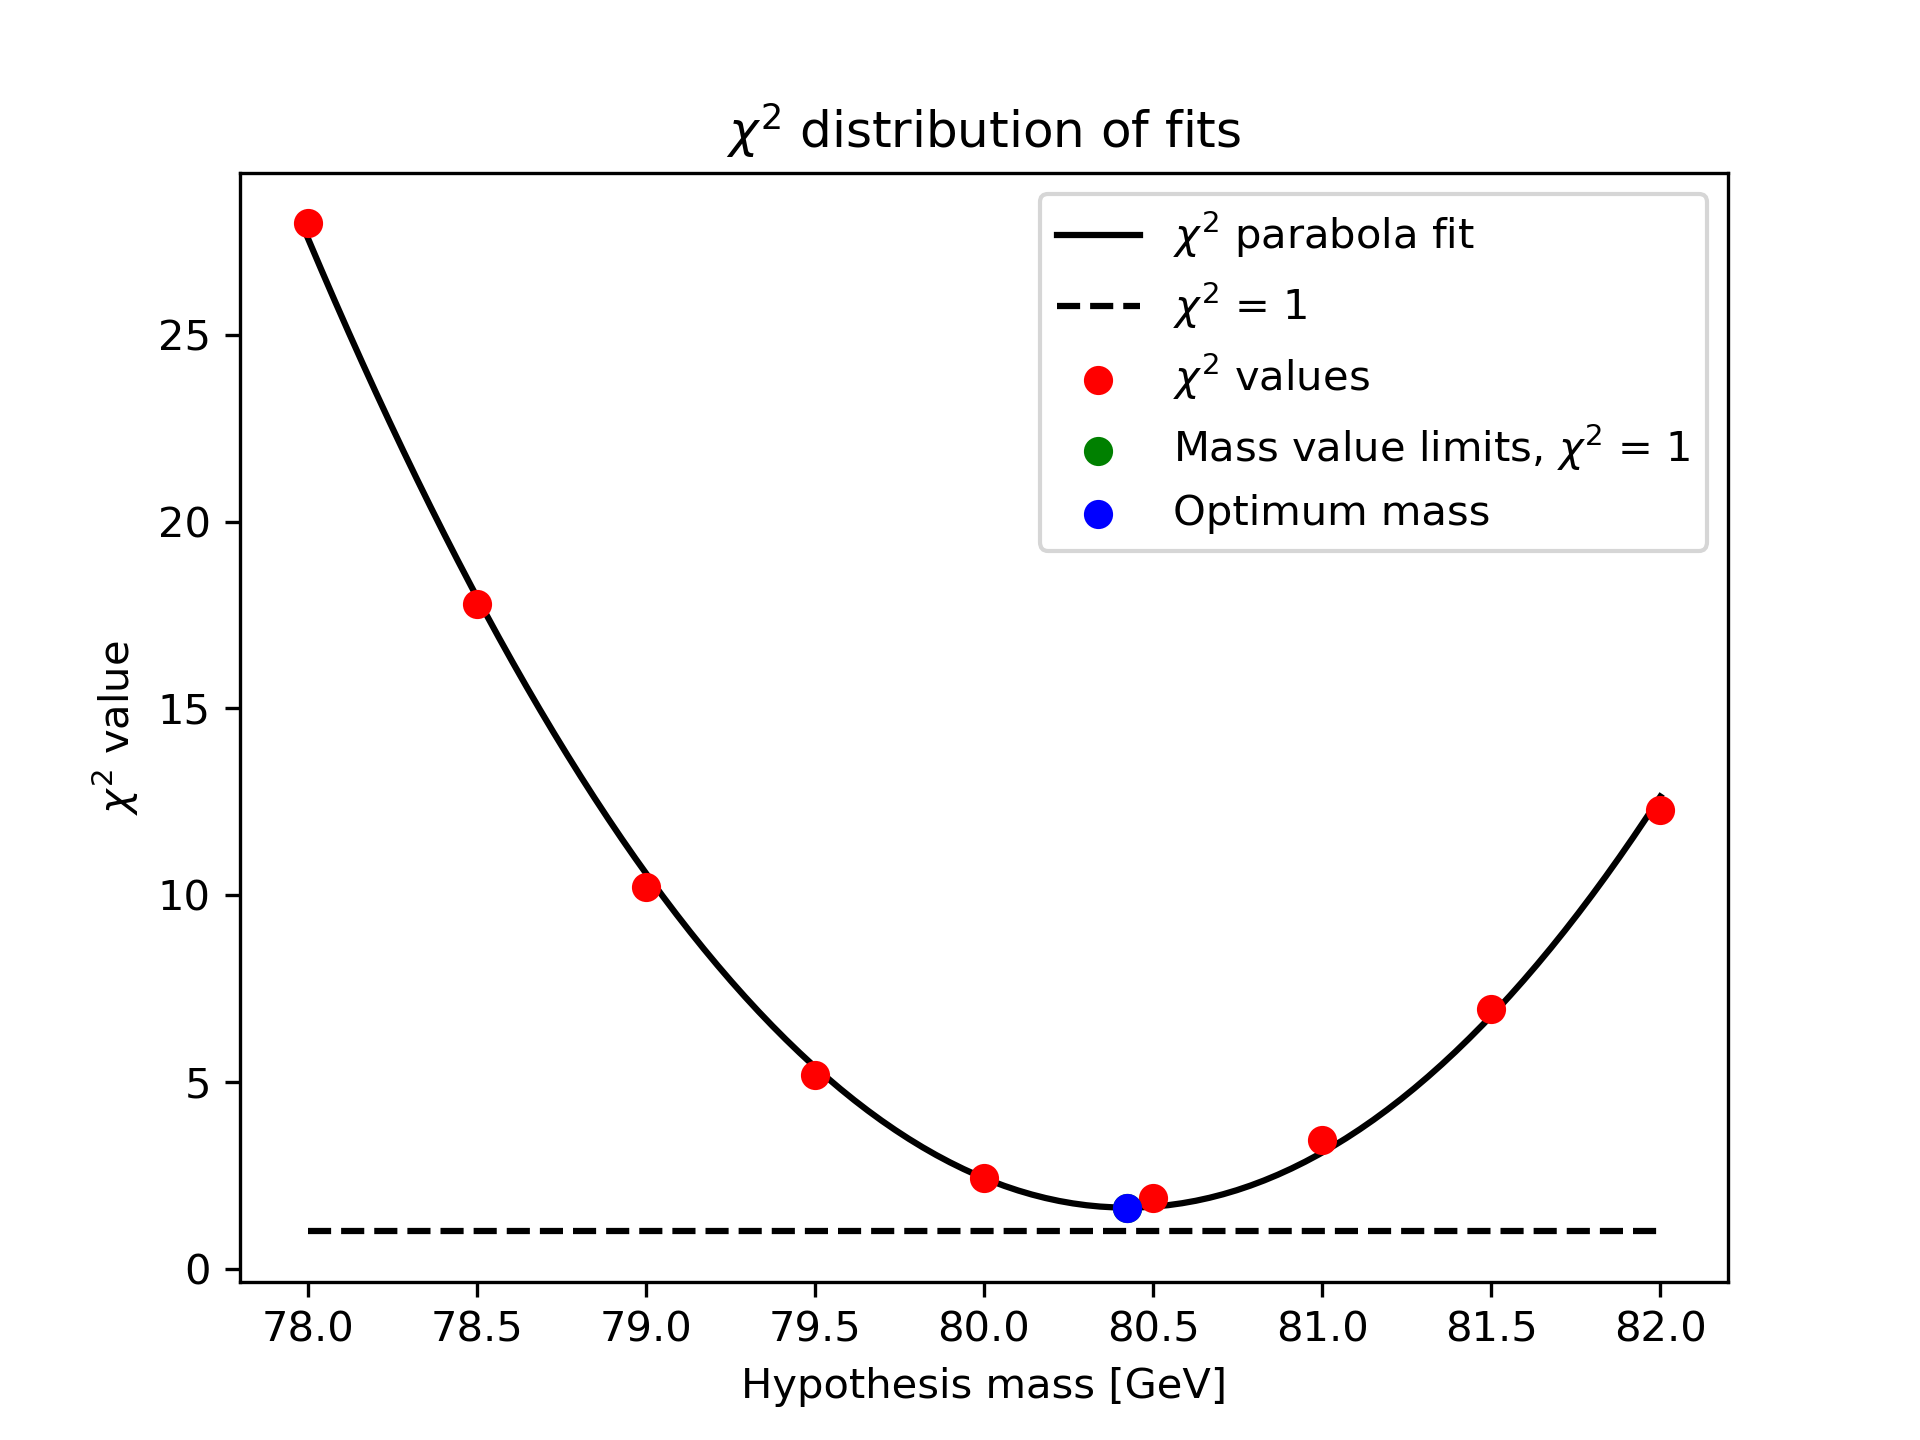
\includegraphics[width=\columnwidth]{/home/physics/phuxdp/Desktop/PX402 Physics Project/WBosonProject/T2W5/plots/chi_square_fits_muPT_80.379_2.07_between_78_and_82_summary.png}
		\caption{\small $\chi^2$ of hypothesis masses. }
		\label{fig: fig_chi_square}
	\end{figure}

    \begin{figure}[tb]
		\centering
		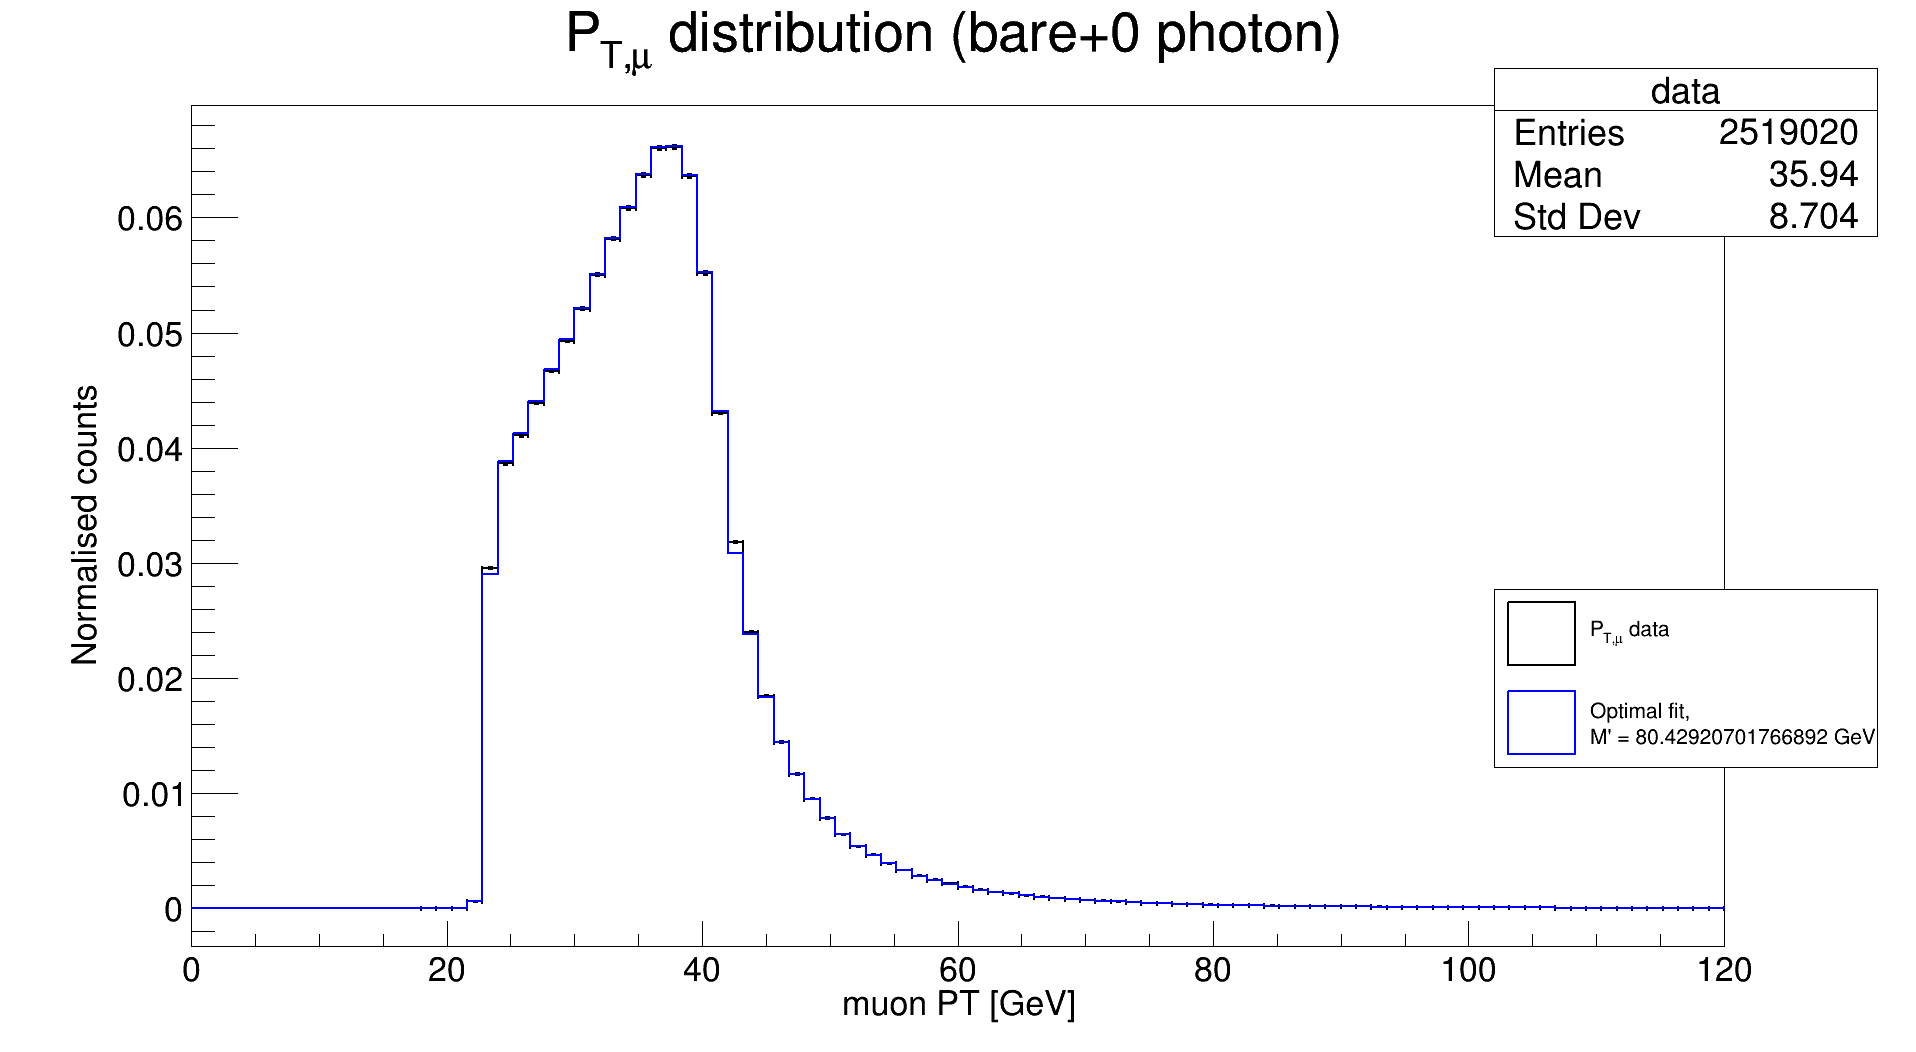
\includegraphics[width=\columnwidth]{/home/physics/phuxdp/Desktop/PX402 Physics Project/WBosonProject/T2W5/plots/optimum_muPT_80.379_2.07_between_78_and_82_summary.png}
		\caption{\small Data and optimum fit with $\chi^2 = 1.0291609941362794$. Used the hypothesis mass of 80.42920701766892$\pm$0.05787070778021075 $[GeV/c^{2}]$. }
		\label{fig: fig_optim_parms}
	\end{figure}
    
\end{document}